\documentclass{article}

\usepackage{graphicx}

\begin{document}

\begin{titlepage}
\title{Searching for circuit complexity lower bounds using SAT solvers}
\author{August Taylor}
\maketitle
\end{titlepage}

\begin{abstract}
Where the abstract will go
\end{abstract}

\tableofcontents

\section{Introduction}

\subsection{Motivation}

Finding lower bounds on the size of Boolean circuits computing given Boolean functions is one of the most fundamental and most challenging problems in computer science. Despite the fact that the majority of functions require exponential circuits, the best lower bounds proven on unrestricted circuits are only linear~\cite{boppana} and we still do not have optimal circuits or close upper and lower bounds for many important functions. Results in this area can be used to separate computational complexity classes, possibly even P and NP (i.e. to show that a large class of fundamental and practically useful problems do not have polynomially fast algorithms).~\cite{arora} 

If functions with circuits of a given complexity could be identified by an efficient algorithm, this could be used to construct efficient learning algorithms for circuits of a smaller complexity; this would resolve one of the biggest questions in learning theory.~\cite{carmosino} Furthermore, such an algorithm could be used to break pseudorandom generators (i.e. distinguish random from pseudorandom inputs).~\cite{arora} As a result, this problem has strong connections in both learning theory and cryptography.

A heuristic approach is to find minimal circuits for small instances of the functions. This can be used to prove new bounds~\cite{kulikovsurvey} and may lead to theoretical insights on the structure of their optimal circuits generally~\cite{williams}. Finding efficient circuits is also necessary in practice when designing electronic systems. 

One approach to automating the search for efficient circuits is to reduce the problem of designing a correct circuit (logical design synthesis) to the Boolean satisfiability problem (SAT). Existing algorithms (SAT solvers) can then be used to solve the problem, either finding a correct circuit of fixed size or generating a proof that none exists~\cite{kulikov}. SAT solvers have become increasingly powerful in recent years *cite* and now have many industrial applications*cite*; the wide range of heuristics implemented by different SAT solvers means that one suited to the problem at hand could be found or developed. *cite* 

*how to extend it*

\subsection{Previous work}

Circuits are a popular model of non-uniform computation. In the past there have been theoretical proofs of lower bounds for restricted circuit classes, e.g. AC0\cite{furst81}\cite{ajtai83}, AC0[k] (i.e. AC0 additionally with MOD-k gates)\cite{razborov87}\cite{smolensky87}, and monotone circuits\cite{razborov85}. However, no lower bounds better than 5n-c\cite{iwama02} have been found for general circuits. Furthermore, there are results stating that it is impossible to use circuit lower bounds to separate P and NP by relativising methods\cite{baker75}, algebrizing methods\cite{aaronson09}, or (under standard crpytpgraphic assumptions) so-called 'natural proofs'\cite{razborov94}. It has been proved that circuit lower bounds are hard to prove using resolution and resolution with k-DNFS, and it is conjectured that they are also hard under stronger proof systems such as Frege systems\cite{raz}. Due to this difficulty in theoretical progress, we would like to investigate the problem empirically.

Kamath et al~\cite{kamath} propose a reduction from logical design synthesis to SAT which fixes the DNF structure of the circuit and number of disjunctions used. Experiments using this reduction to find minimal circuits for 2-4 bit adders and multipliers are reported in~\cite{estrada}. Kojevnikov et al~\cite{kulikov} demonstrate a more general reduction allowing any circuit with a fixed number of gates, proving linear bounds for \(MOD^n_3\) circuits over different Boolean bases. This was done by checking for circuit 'building blocks' with 5 to 11 gates. In~\cite{kulikovlocal} Kulikov et al. used the same reduction to improve large circuit building blocks by searching for smaller versions of their sub-circuits. Specifically, linear upper bounds were proved or verified for \(SUM\), \(MOD^n_4\), and \(MOD^n_3\) by checking for circuits with up to 13 gates (they remarked that checking for existence of a Boolean circuit of size 13 was out of reach).

\subsection{Our contributions}

We investigate feasible ways to find small circuits using SAT reductions. Previous research in this area has focused on a small number of target Boolean functions and a single reduction at a time. Instead, we use multiple combinations of reductions and SAT solvers to see which leads to the best performance. We test them on a range of symmetric functions whose lower bounds are already somewhat understood, in order to analyse the performance in relation to the bound. 

We also search for a general relationship between solver performance and minimum circuit size by applying our methods to a sample of randomly generated functions. We then use solvers to prove a result, that a lower bound conjecture about MOD-3 functions due to Knuth\cite{knuth15} does not hold for the de Morgan basis. 

From these experiments we note that available solvers running on a personal computer can decide the existence of some circuits of size 11 in just a few hours, while others of size 11 and 12 can take many hours on a high-powered computing cluster (13 and above were not investigated). That is to say, the amount of time taken to solve comparable problems can vary considerably.

*Extension axioms - should actually try them first


\section{Background}

\subsection{General setting}

Denote by \(B_{n,m}\) the set of all Boolean functions \(f: \{0,1\}^n \to \{0,1\}^m\) and let \(B_n = B_{n,1}\). A circuit over the basis \(A \subseteq B_2\) is a directed acyclic graph with nodes of in-degree 0 or 2. Nodes of in-degree 0 are called inputs. Nodes of in-degree 2 are assigned functions from \(A\) and are called gates. Some nodes may be also be marked as outputs.

Without loss of generality, we can also assert that every gate has a larger index than both of its predecessors (i.e. the gates are sorted topologically w.r.t. the used numbering); that every gate's second predecessor has a larger index than its first predecessor; and that the last gate is an output.~\cite{kulikov}

A circuit \(c\) of size N is said to compute the function \(f\in B_{n,m}\) if, for all input vectors \(v\in\{0,1\}^n\) in the range of \(f\), \(c(v)=f(v)\), where \(c(v) = (o_1,...o_m)\) are the values of the output gates of \(c\), each input \(x_i\) takes value \(v_i\), and each gate takes the value of its assigned function when applied to the value of its two predecessor nodes.

In this paper, we mainly consider circuits over the De Morgan basis \[C_2 = \{\lor, \land, \neg\}\] where \(\neg\) denotes the Boolean function which outputs the negation of its first argument.

The size of a circuit is its number of gates. We define the circuit existence problem as the question of whether, given a truth table for a function \(f: \{0,1\}^n \to \{0,1\}^m\), there exists a circuit of size N computing \(f\).

\subsection{SAT solvers}

SAT solvers have previously seen success in proving mathematical theorems, most famously in 2016 when Heule et al solved the Boolean Pythagorean Triples problem\cite{heule} and in 2020 when Brakensiek, Heule et al solved Keller's conjecture\cite{heule2}. In general, SAT solvers have the advantage of being effective even when heuristics are not known for solving the original problem, as in the case of circuit existence.

We used three SAT solvers, all based on conflict-driven clause learning. This is an algorithm closely related to DPLL, and which also makes use of the resolution proof system.\cite{cdcl}\cite{krajicek} As mentioned earlier, this means that they cannot decide general circuit lower bounds with a less than exponential-length proof.\cite{raz} However, this asymptotic bound still allows for reasonably-sized proofs for small inputs such as the ones investigated in this paper.

MiniSAT\cite{minisat} was the winner of the 2005 SAT Competition and was last updated to version 2.2 in 2010\cite{minisat2010}. Despite being old, it is well-documented and the other solvers we used were based on it, making it a good baseline for performance. It was also one of the solvers used to decide circuit existence in \cite{kulikov}.

PicoSAT is a solver inspired by miniSAT 1.14, with a focus on improving low-level performance by using optimised data structures\cite{picosat}. It was submitted in the 2010 SAT-Race, and was also one of the solvers used in \cite{kulikov} and the main one in \cite{kulikovlocal}.

MapleSAT is the most recent solver, with variants having won the SAT Competition 2016 and placed second in 2017. It was based off MiniSAT 2.2 but has a different branching heuristic, incorporating ideas from machine learning\cite{maplesat}.

Finally, for use on the Oxford ARC service *fill in the part about glucose-syrup aaaaaaaa*

\subsection{Extension axioms}

\subsection{Reduction to SAT}

We encoded the circuit existence problem as a Boolean formula using three reductions. Let $t$ be the target function with $n$ inputs, and let $N$ be the number of gates required in the circuit.

\subsubsection{Kojevnikov reduction}

The first is due to Kojevnikov et al~\cite{kulikov} who present it together with bounds on the growth rate of the formula. In particular, the growth rate of the number of clauses is $O(N \cdot 2^n)$. The basis of the circuit can be specified as any subset of \(B_2\).

It uses the following variables:

\begin{enumerate}

  \item $t_{ib_1b_2}$ $(n \leq i < n + N, 0 \leq b_1 < 2, 0 \leq b_2 < 2)$ is the value of the $i$-th gate if its first predecessor takes value $b_1$ and its second takes value $b_2$. The four variables $t_{i00}, t_{i01}, t_{i10}, t_{i11}$ thus define the function assigned to the $i$-th gate. This gives $O(N)$ variables.
  \item $c_{ikj}$ $(n \leq i < n + N - 1, 0 \leq k < 2, 0 \leq j < n + N)$ is true iff $j$ is the $k$-th predecessor of $i$. This gives $O(N^2)$ variables.
  \item $o_{ij}$ $(n \leq i < n + N, 0 \leq j < m)$ is true iff the $j$-th output is computed by the $i$-th gate. This gives $O(Nm)$ variables.
  \item $v_{it}$ $(0 \leq i \leq n + N, 0 \leq t < 2^n)$ is the output value of the $i$-th gate if the input variables take values represented by the bits of $t$. These are used to constrain correctness of the circuit on all possible inputs, including its outputs matching the truth table of the encoded function.

\end{enumerate}

We encode the requirements for the circuit by the following clauses:

\begin{enumerate}

  \item The binary function assigned to each gate belongs to our desired basis.
  \item For all $(i,k)$, exactly one variable $c_{ikj}$ is true (there is exactly one $k$-th predecessor of the $i$-th gate). This gives $O(N^3)$ 2-clauses and $O(N)$ $O(N)$-clauses.
  \item For all $j$, exactly one variable $o_{ij}$ is true (the $j$-th output is computed by exactly one gate). This gives $O(N^2m)$ 2-clauses and $O(m)$ $O(N)$-clauses.
  \item For all $0 \leq i < n$ and $0 \leq t < 2^n$, $v_{it}$ is equal to the corresponding bit in $t$. This gives $O(n \cdot 2^n)$ 1-clauses.
  \item For all $n \leq i < n + N$ and $0 \leq t < 2^n$, $v_{it}$ is equal to the value computed by the $i$-th gate. This constrains all the gates with predecessors. Clauses of this type are written for all $n \leq i < n + N$, $n \leq j_0 < i$, $j_0 \leq j_1 < i$, $0 \leq i_0 < 2$, $0 \leq i_1 < 2$, $0 \leq r < 2^n$, and look as follows: 

  \[
    \neg c_{i0j_0} \lor \neg c_{i1j_1} \lor \neg(v_{j_0r} = i_0) \lor \neg(v_{j_1r} = i_1) \lor (v_{ir} = t_{ii_0i_1})
  \]

  This gives $O(N^3 \cdot 2^n)$ 6-clauses.
  \item The outputs of the circuit match the truth table. Clauses of this type are written for all $0 \leq k < m, 0 \leq r < 2^n, n \leq i < n + N$, and look as follows:
 
  \[
    \neg o_{ik} \lor (v_{ir} = value_{kr})
  \] 

  where $value_{kr}$ is the required value of the $k$-th output when the circuit is given input $r$, according to the truth table. This gives $O(N2^nm)$ clauses.

\end{enumerate}


\subsubsection{Razborov reduction}

The second is due to Razborov~\cite{raz}, assumes the function outputs only a single Boolean value, and requires a circuit over the basis \(C_2\). Note that it has a lower growth rate (in terms of number of clauses) than the other two reductions - $O(N \cdot 2^n)$ as opposed to $O(N^3 \cdot 2^n)$ - suggesting it encodes the requirements more efficiently.

It uses the following variables:

\begin{enumerate}

  \item $y_{av}$ $(a \in {0,1}^n, v \in [N])$ is the value taken by node $v$ on circuit input $a$. This gives $O(N \cdot2^n)$ variables.
  \item $y_{a\nu v}$ $(a \in {0,1}^n, \nu \in {1,2}, v \in [N])$ is the value of the $\nu$-th predecessor to $v$ on input $a$. This gives $O(N \cdot 2^n)$ variables.
  \item $Fanin(v)$ is 0 if $v$ is a $\neg$-gate and 1 otherwise. This gives $O(N)$ variables.
  \item $Types(v)$ - when $Fanin(v)=1$, this is 0 if $v$ is a $\land$-gate and 1 if $v$ is a $\lor$-gate. This gives $O(N)$ variables.
  \item $InputType_\nu(v)$ is 0 if the $\nu$-th predecessor to $v$ is a constant or an input, 1 if it is another gate. This gives $O(N)$ variables.
  \item $InputType'_\nu(v)$ - when $InputType_{\nu}(v) = 0$, this is 0 if the $\nu$-th predecessor to $v$ is a constant, 1 if it is an input. This gives $O(N)$ variables.
  \item $InputType''_\nu(v)$ - when $InputType_{\nu}(v) = InputType'_{\nu}(v) = 0$, this is the value of the constant $\nu$-th predecessor to $v$. This gives $O(N)$ variables.
  \item $InputVar_\nu(v,i)$ $(i \in [n])$ - when $InputType_{\nu}(v) = 0, InputType'_{\nu}(v) = 1$, this is 1 iff the $\nu$-th predecessor to $v$ is the $i$-th input. This gives $O(N \cdot n)$ variables.
  \item $INPUTVAR_\nu(v,i)$ is equal to $\bigvee_{i'<i} InputVar_\nu(v,i')$, which will be used to bound the fan-in below. This gives $O(N \cdot n)$ variables.
  \item $InputNode_\nu(v,v')$ $(v' < v)$ - when $InputType_{\nu}(v) = 1$, this is 1 iff $\nu$-th predecessor to $v$ is the gate $v'$. This gives $O(N^2)$ variables.
  \item $INPUTNODE_\nu(v,v')$ is analogous to $INPUTVAR_\nu(v,i)$. This gives $O(N^2)$ variables.
  
\end{enumerate}

We encode the requirements for the circuit by the following expressions:

\begin{enumerate}

  \item Constant predecessors take the correct values, giving $O(N)$ clauses:

  $\neg InputType_\nu(v) \land \neg InputType'_\nu(v) \rightarrow (y_{a \nu v} = InputType''_\nu(v))$

  \item Gates have at most one input per input predecessor, giving $O(N \cdot n^2)$ clauses:

  $\neg InputType_\nu(v) \land InputType'_\nu(v) \rightarrow \neg (InputVar_\nu(v,i) \land InputVar_\nu(v,i'))$ for $i \neq i'$

  \item INPUTVAR variables take the correct value, giving $O(N \cdot n)$ clauses:

  $\neg InputType_\nu(v) \land InputType'_\nu(v) \rightarrow (INPUTVAR_\nu(v,i) = (InputType_\nu(v),i-1) \lor InputVar_\nu(v,i)))$, where $InputType_\nu(v,0) = 0$

  \item Gates have at least one input per input predecessor, giving $O(N)$ clauses:

  $\neg InputType_\nu(v) \land InputType'_\nu(v) \rightarrow INPUTVAR_\nu(v,n)$

  \item Input predecessors take the correct values, giving $O(N \cdot n \cdot 2^n)$ clauses:

  $\neg InputType_\nu(v) \land InputType'_\nu(v) \land InputVar_\nu(v,i) \rightarrow (y_{a \nu v} = a_i)$

  \item The analogous clauses to the above, but for InputNode and gate predecessors. 

  \item Gates take the correct value, giving $O(N \cdot 2^n)$ clauses.

  \item The final gate (i.e. the output) matches the truth table, giving $O(2^n)$ clauses.

\end{enumerate}

\subsubsection{Naive reduction}

The third reduction is straightforward. It also assumes the function outputs only a single Boolean value and requires a circuit over the basis \(C_2\). The growth rate for the number of clauses is $O(N \cdot 2^n)$, the same as for the Kojevnikov reduction.

It uses the following variables:

\begin{enumerate}
  \item \(e^i_a\) \((n \leq i < N, a\in\{0,1\}^n)\) is the value of the \(i\)-th gate when the input to the circuit is \(a\). This gives \(O(N \cdot 2^n)\) variables.
  \item \(x_{i,j}\) \(( 0 \leq i < N+n,0 \leq j < i)\) is true iff j is a predecessor of i. This gives \(O(N \cdot (N+n))\) variables.
  \item \(g^0_i, g^1_i\) \((n \leq i < N)\) together encode the function assigned to the \(i\)-th gate by their truth values, giving \(2N\) variables:

    \begin{center}
    \begin{tabular}{ |c|c|c| }
    \hline
    \(g^0_i\) & \(g^1_i\) & Function \\ 
    \hline
    0 & 0 & \(\neg\) \\  
    0 & 1 & \(\lor\) \\ 
    1 & 0 & \(\land\) \\ 
    1 & 1 & \(\neg\) \\   
    \hline
    \end{tabular}
    \end{center}

\end{enumerate}

We encode the requirements for the circuit by the following clauses:

\begin{enumerate}
  \item For all \((i,j,k)\) with \(n \leq i < n+N\), \(0 \leq j < i\) and \(j < k < i\), and for all \(a\in\{0,1\}^n\), if \(j\) and \(k\) are both predecessors of \(i\), then \(e^i_a\) must take the value computed by the \(i\)th gate's assigned function on \(e^j_a\) and \(e^k_a\). Clauses must be added for each function in the basis. For example, the expression for when the \(i\)th gate is an \(\land\)-gate:

\[
(g^0_i\wedge \neg g^1_i)\wedge 
(x_{i,j}\wedge x_{i,k})\rightarrow 
(e^i_a\leftrightarrow e^j_a\wedge e^k_a)
\]
  
  Note that the gate must compute the conjunction of any two predecessors' variables. This means it can have at most two predecessors, otherwise the conjunctions of different pairs of predecessors may disagree and the gate will have no correct value. This gives \(O(2^n\cdot N^3)\) 7-clauses.

  \item For all \(i\) with \(n \leq i < n+N\), gate \(i\) must have at least one predecessor. This gives \(O(N)\) \(O(N+n)\)-clauses.

  \item For all \((i,j)\) with \(n \leq i < n+N\), \(0 \leq j < i\), if \(i\) is an \(\lor\)-gate or \(\land\)-gate with \(j\) its predecessor, it must have another distinct predecessor (i.e. it must have at least 2 overall). For example, the expression for when the \(i\)th gate is an \(\land\)-gate:

\[
(g^0_i \land \neg g^1_i) \rightarrow \left( x_{i,j} \rightarrow \bigvee_{j<k<i} x_{i,k} \right)
\]

  This gives \(O(N^2)\) \(O(N)\)-clauses.

  \item For all \(i\) with \(0 \leq i < n\), \(a\in\{0,1\}^n\), the \(i\)-th input must equal \(a_i\). This gives \(O(n \cdot 2^n)\) 1-clauses.

  \item For all \(a\in\{0,1\}^n\), the final m gates (i.e. the outputs) should agree with the output values given for \(a\) in the target truth table. This gives \(O(2^n)\) 1-clauses.

\end{enumerate}

\section{Results}

Timed experiments were carried out on a 3.400GHz Intel i3-8130U processor running Linux. The times shown were obtained by running the software on the problem 3 times and taking the median.

Further experiments were conducted on the Oxford ARC service *cite* using 1 node which could run up to 32 processes in parallel. *add more details about ARC pleas

\subsection{Comparison of Boolean functions}\label{funcresults}

We investigated the relationship between the size of a circuit and the time taken for a SAT solver to confirm or deny its existence. We encoded a range of simple symmetric functions using the Kulikov encoding:

\begin{enumerate}
  \item AND on 7-bit and 8-bit inputs
  \item Parity on 3-bit and 4-bit inputs
  \item \(MOD^0_3\) and \(MOD^0_4\) on 3-bit and 4-bit inputs
  \item Majority on 3-bit and 4-bit inputs
  \item Partial parity - *Explain why partial functions are useful for encoding lower bounds on big input-lengths. But also need to find a way to get good data for them (ie. more than 1 second per problem...)

\end{enumerate}

We chose to investigate the existence of circuits up to 9 gates, as these were reliably solved within less than 9 hours on the single-processor hardware described.

The size of the minimal circuit is shown in red*need to re-plot the graphs to make this work better*. It was found that the time needed to solve a problem tended to spike on or around the optimal circuit size. This may be because it is difficult to confirm or rule out circuits that come close to satisfying the requirements. Another possibility is that when close to the optimal size, there is the lowest proportion of satisfying circuits relative to the total amount of possible circuits, meaning that more of the search space must be explored (as opposed to quickly exploring it all at small sizes or quickly landing upon a satisfying circuit at large sizes). A similar phenomenon was reported in~\cite{estrada}. 

Different functions took different amounts of time overall, varying between seconds and hours, something also seen in Section \ref{randomresults}. Performance for each function was not especially consistent between the solvers; usually they found the same things difficult, but the length of time each solver took for the difficult problems varied, for example in \ref{fig:8andkulikov} or. The extent of this can be seen in Section \ref{satresults}.

A complete display of graphs can be found in the appendix.

\begin{figure}[!ht]
  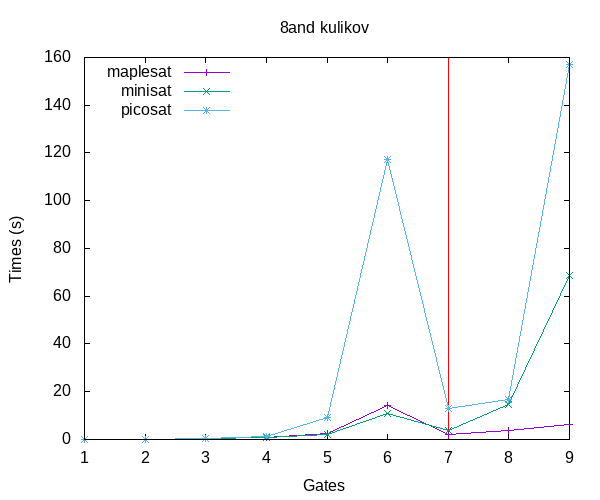
\includegraphics[width=\textwidth]{images/times/8andkulikov.png}
  \label{fig:8andkulikov}
  \caption{Times taken by SAT solvers to check for existence of a circuit computing AND on 8 bits}
\end{figure}

\begin{figure}[!ht]
  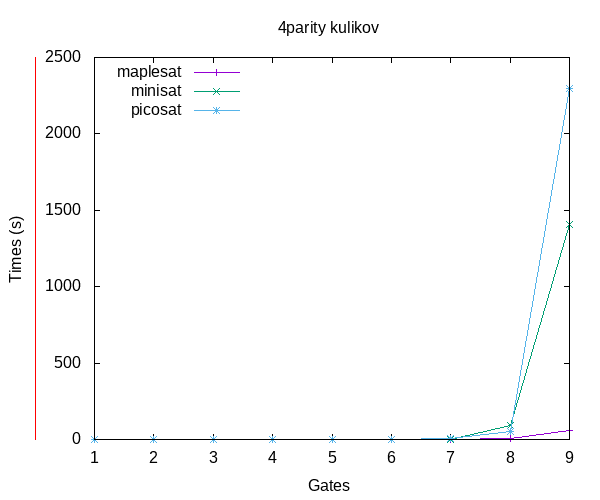
\includegraphics[width=\textwidth]{images/times/4paritykulikov.png}
  \label{fig:4paritykulikov}
  \caption{Times taken by SAT solvers to check for existence of a circuit computing parity on 4 bits}
\end{figure}

\subsection{Comparison of SAT solvers and reductions} \label{satresults}

We investigated whether there was a relationship between the reduction used to encode a Boolean function, the solver used, and the time taken by the solver. We took the total of the times each combination took to solve the problems from Section \ref{funcresults} and compared them as shown in \ref{totals}.

\begin{figure}[!ht]
  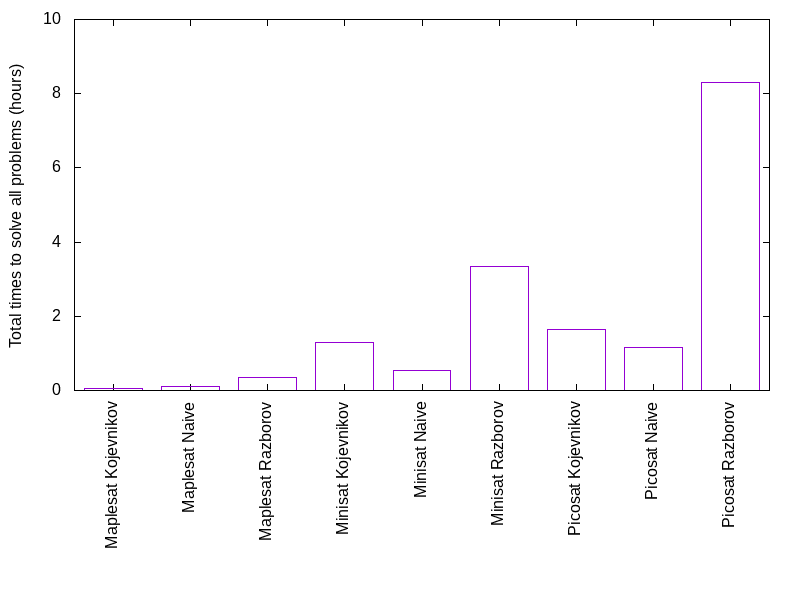
\includegraphics[width=\textwidth]{images/totals.png}
  \label{fig:totals}
  \caption{Comparison of times taken by SAT solvers on different reductions}
\end{figure}

It can be seen that MapleSAT on the Kulikov encoding performs the best. Apart from this, the effect of the reduction and the solver seem to be independent, with MapleSAT consistently performing better than MiniSAT and PicoSAT, and the Naive and Kojevnikov reductions performing better than the Razborov reduction. It is possible that the efficient encoding of the Razborov reduction is detrimental to the performance of the solver. However, these results are only applicable to small values of n. **however I should take out the constants and re-run the experiments to be sure it’s not that..

\subsection{Random functions}\label{randomresults}

64 truth tables were generated for 4-bit inputs using a pseudorandom number generator simulating a uniform distribution (specifically, xorshift128+ due to the TypeScript implementation). The existence of circuits of size 1 to 11 for these tables were encoded with the Kojevnikov reduction and solved using MapleSAT. The times taken to check for circuits are shown plotted against their optimal circuit size in \ref{fig:4rand_scatter} (note that 2 tables could not be fully solved within 9 hours; these functions have been omitted leading to a sample size of 62). The distribution of optimal circuit sizes is shown in \ref{fig:4rand_sizes}.

The scatter graph shows a clustering in times between functions of the same optimal circuit size, but with a few outliers taking more time. This is most easily seen for sizes 10 and 11 (although the same is visible for 8 and 9 when plotted on a smaller scale). Also, the clustered functions of each optimal circuit size took strictly less time to solve than those with larger sizes, despite the fact that we always checked for existence up to 11 gates. This shows a generally strong relationship between the difficulty of checking circuit existence and the complexity of the function.

While we expect a large proportion of circuits to be hard (i.e. have a large optimal circuit size) for large input sizes~\cite{arora}, the usual counting arguments break down for such small values of n. However, using the SAT solver we can check the number of hard circuits directly. While the small sample size can account for the irregular shape of the graph in \ref{fig:4rand_sizes}, there does appear to be a peak around 10 gates. This contradicts the intuition that there should be exponentially more harder functions, and suggests that there is quite a low upper limit on the complexity of a function which only can only vary over 4 bits of input. However, this is all under the assumption that the pseudorandom generator used did output a truly random sample; in reality, it may have sampled disproportionately many easy (or hard) functions.

\begin{figure}[!ht]
  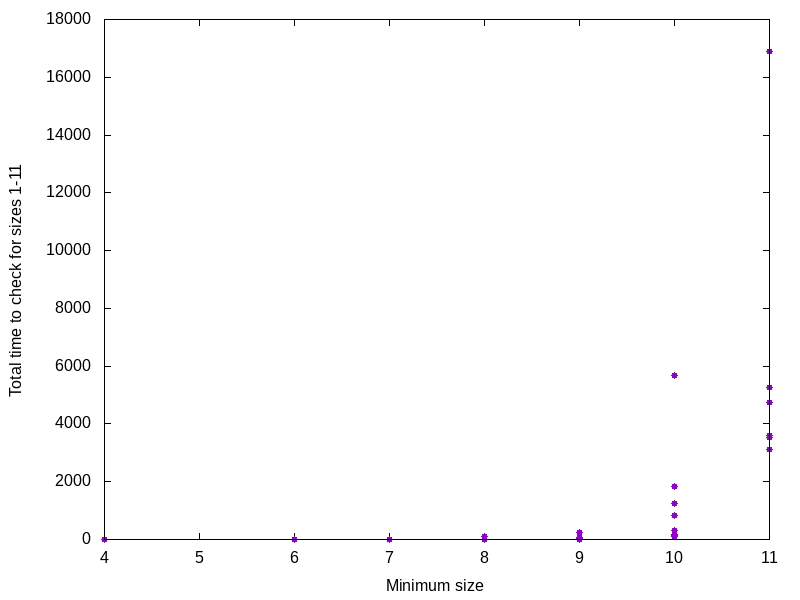
\includegraphics[width=\textwidth]{images/random/4bit_scatter.png}
  \label{fig:4rand_scatter}
  \caption{Time taken to check up to 11 gates for randomly chosen functions *still need to plot on some of the symmetric functions*}
\end{figure}
\begin{figure}[!ht]
  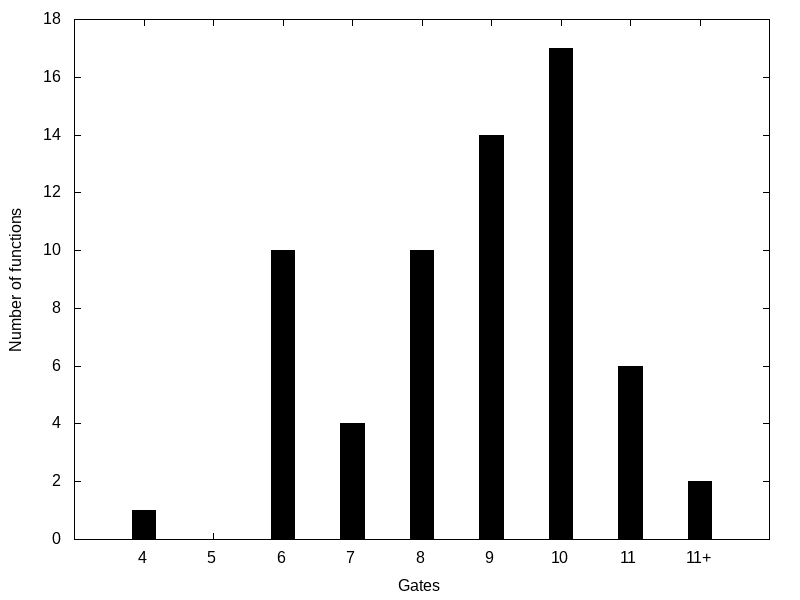
\includegraphics[width=\textwidth]{images/random/4bit_sizes.png}
  \label{fig:4rand_sizes}
  \caption{Sizes of optimal circuits for 4-bit functions with randomly chosen truth tables}

\end{figure}

\subsection{Knuth's MOD-3 conjecture}

\subsection{Extension axioms}

\section{Discussion}

\subsection{Summary}
section to be included if I need to get closer to 10,000 words :)

\subsection{Reflection}

The main practical lesson learned from this project was to think in the long term. Firstly, by writing code that can easily be adapted, i.e. following good OOP practices and providing a flexible interface for conducting experiments from the start, so that less refactoring will be needed later. Also, by writing code that can scale to dealing with larger numbers as the scope and ambition of the project expands. This could be done by choosing a well-suited programming language, algorithms and data structures - I chose TypeScript and used arrays as these were familiar and easy to get started with, and the performance of my code and poor documentation of the different pseudorandom generators in the language was an unexpected barrier later on.

describe the general timeline of the project and the different things I implemented that didn't make it into the final, mistakes I made with initial experiments, etc. towards the end would have been better to envision the final experiments and how to get the best results rather than focusing immediately on getting things to work.

things to mention that are not practical - more of how to read papers and do background reading, about how SAT solvers work and their applications, about the state of circuit bounding and P vs NP, the creative process of working on a research project with a lot of backtracking, etc.

\subsection{Conclusions}

\subsection{Further directions}
-Search for the circuit size for literally all 4-bt funcitons (or bigger eg. maybe 9 bits will allow the bounding trick to apply)

\bibliographystyle{plain} 
\bibliography{sources}

\end{document}